% Options for packages loaded elsewhere
\PassOptionsToPackage{unicode}{hyperref}
\PassOptionsToPackage{hyphens}{url}
%
\documentclass[
]{article}
\usepackage{amsmath,amssymb}
\usepackage{lmodern}
\usepackage{iftex}
\ifPDFTeX
  \usepackage[T1]{fontenc}
  \usepackage[utf8]{inputenc}
  \usepackage{textcomp} % provide euro and other symbols
\else % if luatex or xetex
  \usepackage{unicode-math}
  \defaultfontfeatures{Scale=MatchLowercase}
  \defaultfontfeatures[\rmfamily]{Ligatures=TeX,Scale=1}
\fi
% Use upquote if available, for straight quotes in verbatim environments
\IfFileExists{upquote.sty}{\usepackage{upquote}}{}
\IfFileExists{microtype.sty}{% use microtype if available
  \usepackage[]{microtype}
  \UseMicrotypeSet[protrusion]{basicmath} % disable protrusion for tt fonts
}{}
\makeatletter
\@ifundefined{KOMAClassName}{% if non-KOMA class
  \IfFileExists{parskip.sty}{%
    \usepackage{parskip}
  }{% else
    \setlength{\parindent}{0pt}
    \setlength{\parskip}{6pt plus 2pt minus 1pt}}
}{% if KOMA class
  \KOMAoptions{parskip=half}}
\makeatother
\usepackage{xcolor}
\usepackage[margin=1in]{geometry}
\usepackage{longtable,booktabs,array}
\usepackage{calc} % for calculating minipage widths
% Correct order of tables after \paragraph or \subparagraph
\usepackage{etoolbox}
\makeatletter
\patchcmd\longtable{\par}{\if@noskipsec\mbox{}\fi\par}{}{}
\makeatother
% Allow footnotes in longtable head/foot
\IfFileExists{footnotehyper.sty}{\usepackage{footnotehyper}}{\usepackage{footnote}}
\makesavenoteenv{longtable}
\usepackage{graphicx}
\makeatletter
\def\maxwidth{\ifdim\Gin@nat@width>\linewidth\linewidth\else\Gin@nat@width\fi}
\def\maxheight{\ifdim\Gin@nat@height>\textheight\textheight\else\Gin@nat@height\fi}
\makeatother
% Scale images if necessary, so that they will not overflow the page
% margins by default, and it is still possible to overwrite the defaults
% using explicit options in \includegraphics[width, height, ...]{}
\setkeys{Gin}{width=\maxwidth,height=\maxheight,keepaspectratio}
% Set default figure placement to htbp
\makeatletter
\def\fps@figure{htbp}
\makeatother
\setlength{\emergencystretch}{3em} % prevent overfull lines
\providecommand{\tightlist}{%
  \setlength{\itemsep}{0pt}\setlength{\parskip}{0pt}}
\setcounter{secnumdepth}{-\maxdimen} % remove section numbering
\usepackage[width=\textwidth]{caption}
\ifLuaTeX
  \usepackage{selnolig}  % disable illegal ligatures
\fi
\IfFileExists{bookmark.sty}{\usepackage{bookmark}}{\usepackage{hyperref}}
\IfFileExists{xurl.sty}{\usepackage{xurl}}{} % add URL line breaks if available
\urlstyle{same} % disable monospaced font for URLs
\hypersetup{
  pdftitle={Increase Variation Around Narrow ESD Concepts},
  hidelinks,
  pdfcreator={LaTeX via pandoc}}

\title{Increase Variation Around Narrow ESD Concepts}
\author{}
\date{\vspace{-2.5em}}

\begin{document}
\maketitle

The quantitative benchmarks of ESDs are meant to capture the variation
inherent in a state and phase under multiple conditions, from
consecutive drought to surpluses of moisture, and following multiple
disturbances (CITE). They are intended to capture the variation that
would be found in this state and phase combination across the geographic
and climatic extents of the ESD in the relevant MLRA. Some of the
quantitative benchmarks, of the fractional cover of functional
vegetation groups, for Ecological Sites which we collected from ESD's
were very narrow. In many of these instances the reported values were
more narrow than the uncertainty of the estimates of the true value of
the population gleaned from a single AIM plot. It is apparent that
several ESD developers did not emphasize the natural variability of the
vegetation benchmarks while generating the cover estimates. This may be
due to them only collecting quantitative vegetation data at a single
site, and not across multiple time points, accordingly it seems in
multiple instances they may only have had a point of datum, and did not
feel comfortable estimate the variation in the system.

Well that approach is prudent, it is not prudent for us to assume such
narrow ranges of variation. These may unduly penalize estimates of the
amount of land under analysis which are meeting condition benchmarks.
Here we seek to identify and broaden these estimates, we will use a
simple method of \emph{imputing} values in the context of \emph{feature
engineering}. A \emph{linear model} will be fit to the benchmark values,
which contain realistic ranges, and then the slope of this model will be
used to fill in the missing values.

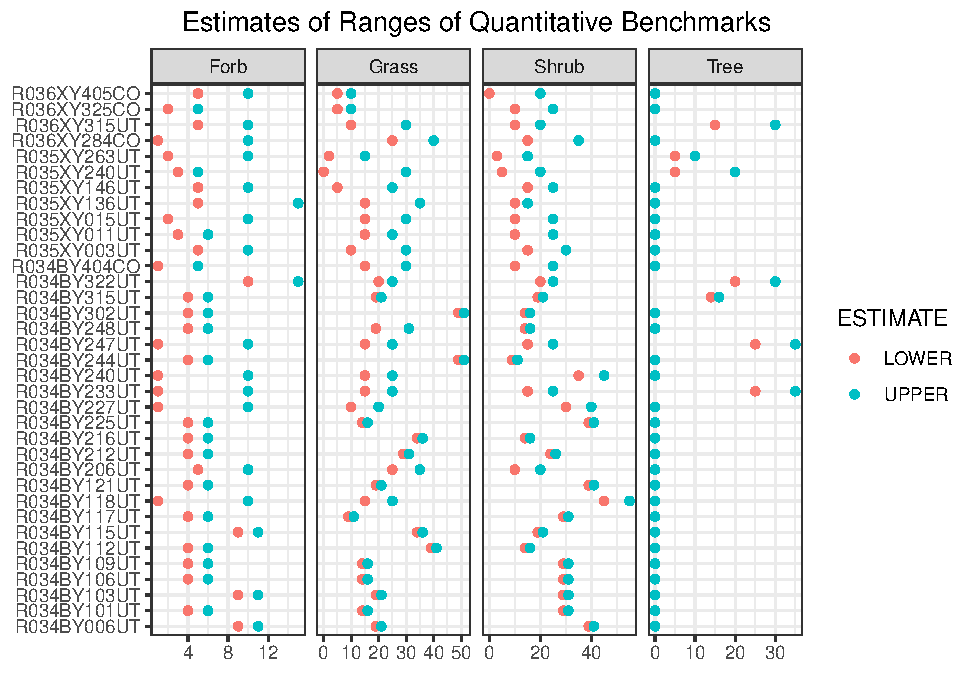
\includegraphics{increase_range_around_narrow_means_files/figure-latex/Plot Initial variation-1.pdf}

Ranges of estimated benchmark variation were estimated as being too low
if they fell within the ranges in Table 1 \& Figure 1 \emph{top panel}.
These XX values were removed from the initial data set. The remaining XX
observations were used as \textbf{training} data for the linear models.
Once the linear model was \emph{fitted}, the removed data points had
estimates of their values recorded.

\begin{longtable}[]{@{}cc@{}}
\toprule()
Mean & Range \\
\midrule()
\endhead
\textless{} 10 & \textless{} 3 \\
10 - 20 & \textless{} 4 \\
20 - 30 & \textless{} 5 \\
30 - 50 & \textless{} 6 \\
\bottomrule()
\end{longtable}

\(\text{Range} \sim \text{Mean + Functional Group}\)

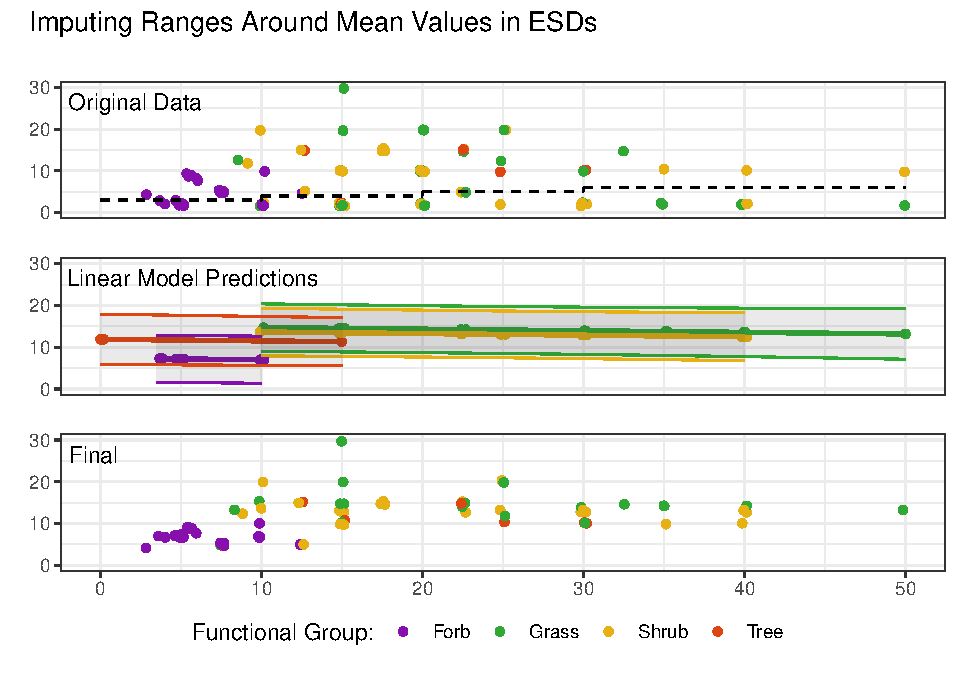
\includegraphics{increase_range_around_narrow_means_files/figure-latex/unnamed-chunk-1-1.pdf}

\end{document}
